\section{Numerical implementations using standard finite elements}

\subsection{Comparison of the micromorphic solutions to the phase-field solutions on selected test cases  using \texttt{mgis.fenics}}
\label{sec:micromorphicdamage:test_cases}

In this section, the
\texttt{mgis.fenics}
% (https://thelfer.github.io/mgis/web/mgis_fenics.html)
% python module is used \cite{bleyer_overview_2020}


We consider in this section three classical test cases:

\begin{itemize}
  \item a fiber reinforced matrix in tension, as proposed in \cite{bourdin_numerical_2000}
  \item a precracked specimen loaded by applying a tangential displacement on
  the top boundary, as proposed in \cite{miehe_phase_2010}
  \item a precracked specimen loaded by applying a normal displacement on the
  top boundary, as proposed by \cite{miehe_phase_2010}
\end{itemize}


\begin{figure}[H]
  \centering
  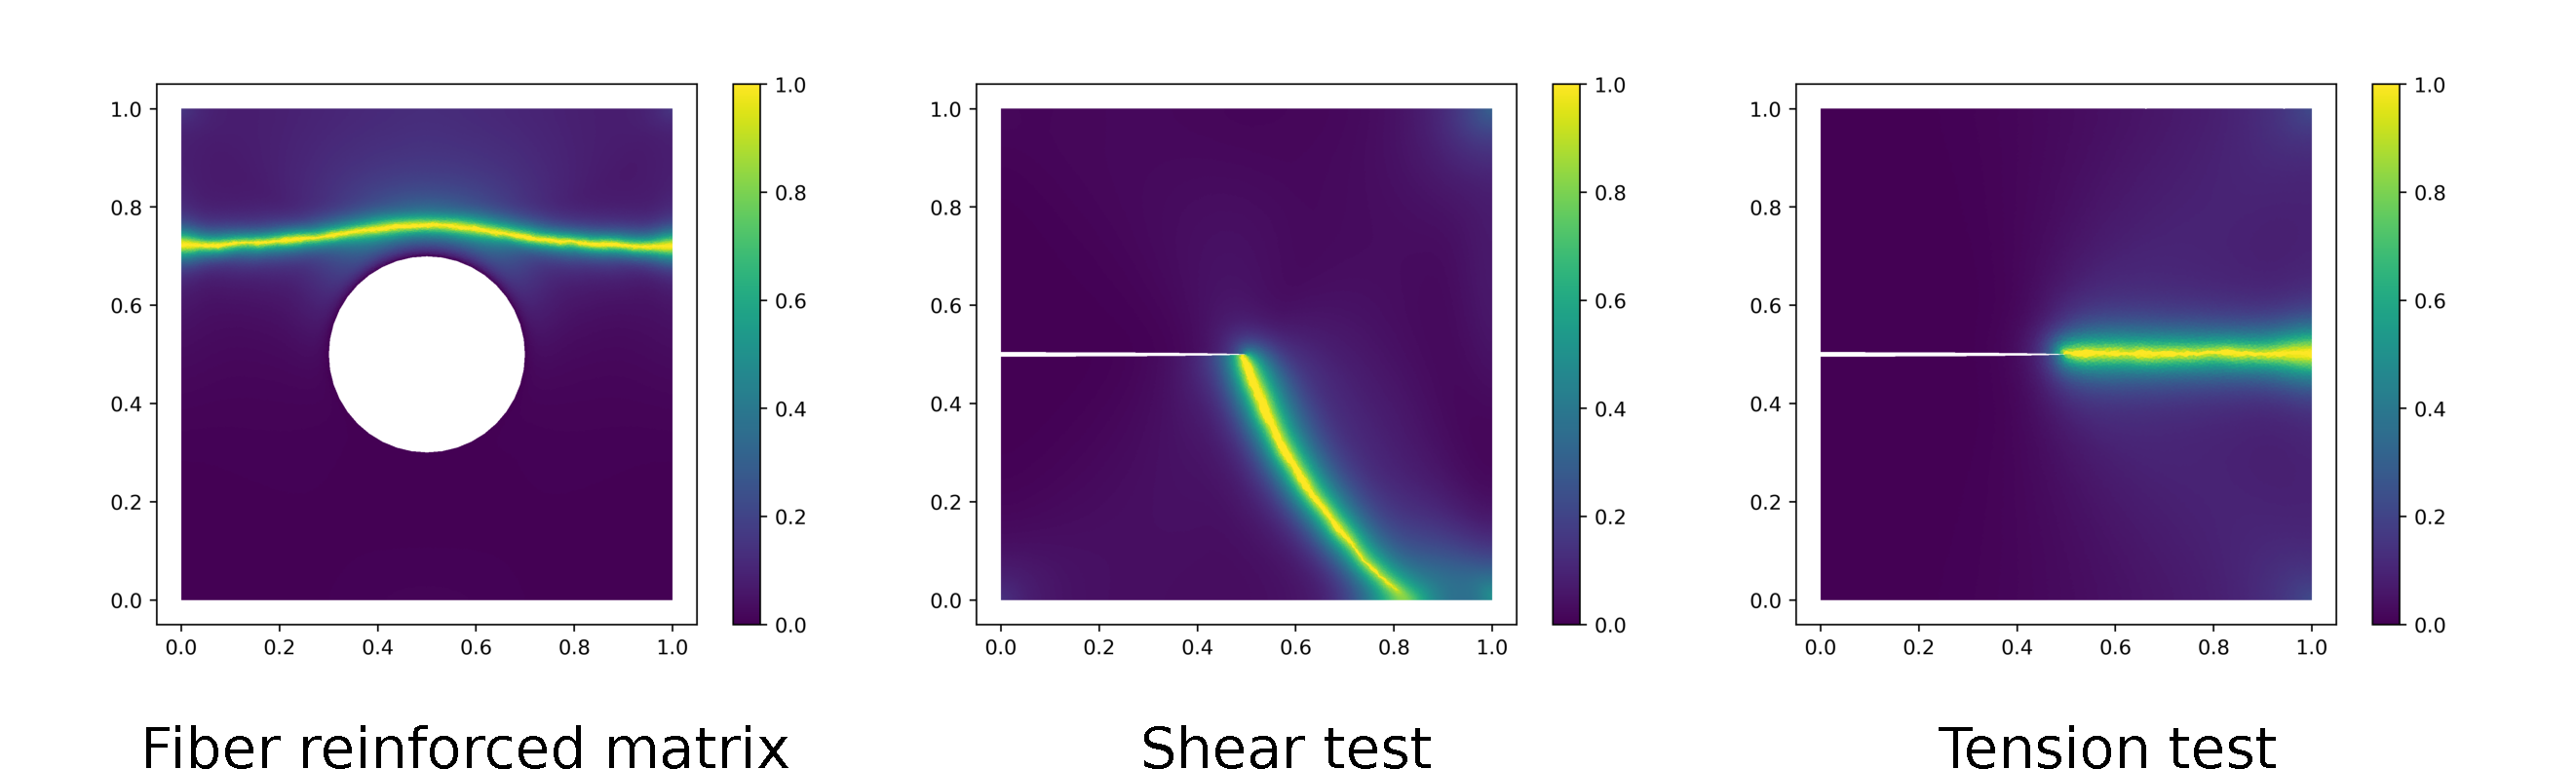
\includegraphics[width=10.cm]{../chapter_02_ef_micromorphic/figures/DamagePattern.pdf}
  \caption{Damage patterns at the end of the unit tests}
  \label{fig:micromorphicdamage:damage_patterns}
\end{figure}

% ![Damage patterns at the end of the unit tests.](img/DamagePattern.pdf){#fig:micromorphicdamage:damage_patterns}

Those tests are performed using the AT2 model and its micromorphic
counterparts using a spectral decomposition of the elastic free energy.
The damage patterns at the end of those tests are reported on Figure
\ref{fig:micromorphicdamage:damage_patterns}.

The \texttt{python} scripts are available in this repository:
https://github.com/thelfer/micromorphic-damage-giens-2022.

Those scripts contains the geometry, material properties and loadings
required to reproduce those tests.

For those tests, the penalisation parameter \(H_{\chi}\) is chosen of
the form:
\[
H_{\chi}= \beta\,\Frac{G_{c}}{l_{0}}
\]

where \(\beta\) is a normalised penalisation parameter \cite{bharali_computational_2021}.

\subsection{Choice of the convergence criterion of the staggered schemes}

In this paper, the staggered schemes are stopped when the damage becomes
stationnary, i.e. when the absolute difference between two estimates of
the damge is below a given threshold \(\varepsilon_{d}\) at each
integration point.

This criterion is not totally satisfying as it does not ensure that a
true minimun of the Lagrangian is found. We carefully checked that this
is the case for each steps of the numerical experiments described in
this section.

\subsection{Discussion}

Those three tests lead to similar conclusions:

% ![Evolution of the force as a function of the imposed displacement for
% the fiber reinforced matrix test for the third scheme with \(\beta=150\)
% and the standard phase-field schemes based on the resolution of the
% variational inegality or based on Miehe' history
% function](img/FiberReinforcedMatrix-force.pdf){#fig:micromorphic_damage:force
% width=75%}

\begin{figure}[H]
  \centering
  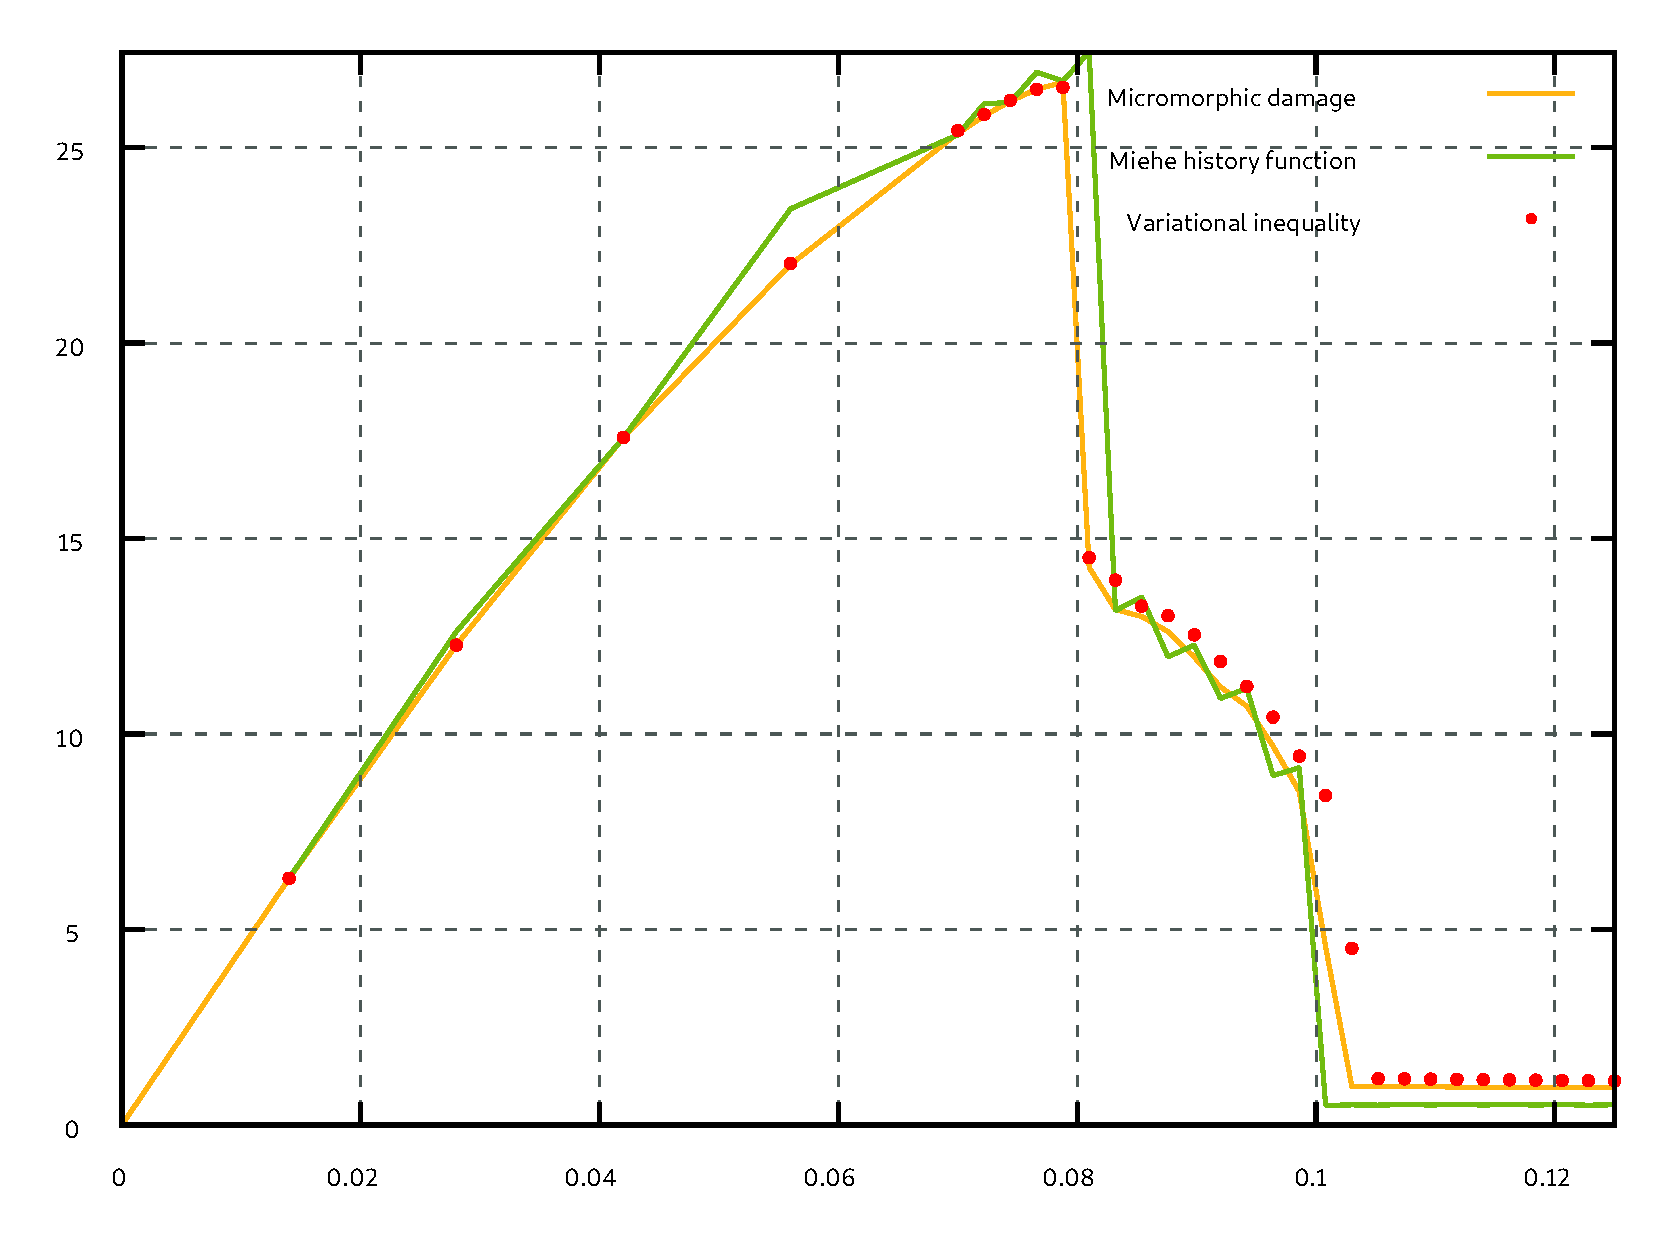
\includegraphics[width=10.cm]{../chapter_02_ef_micromorphic/figures/FiberReinforcedMatrix-force.pdf}
  \caption{Evolution of the force as a function of the imposed displacement for
  the fiber reinforced matrix test for the third scheme with \(\beta=150\)
  and the standard phase-field schemes based on the resolution of the
  variational inegality or based on Miehe' history
  function}
  \label{fig:micromorphic_damage:force}
\end{figure}

% ![Evolution of the force as a function of the imposed displacement for
% \(\beta=50\), \(\beta=100\), \(\beta=150\) for the shear test using the
% third staggered scheme.](img/shear-force.pdf){width=75%
% #fig:micromorphic_damage:beta}

\begin{figure}[H]
  \centering
  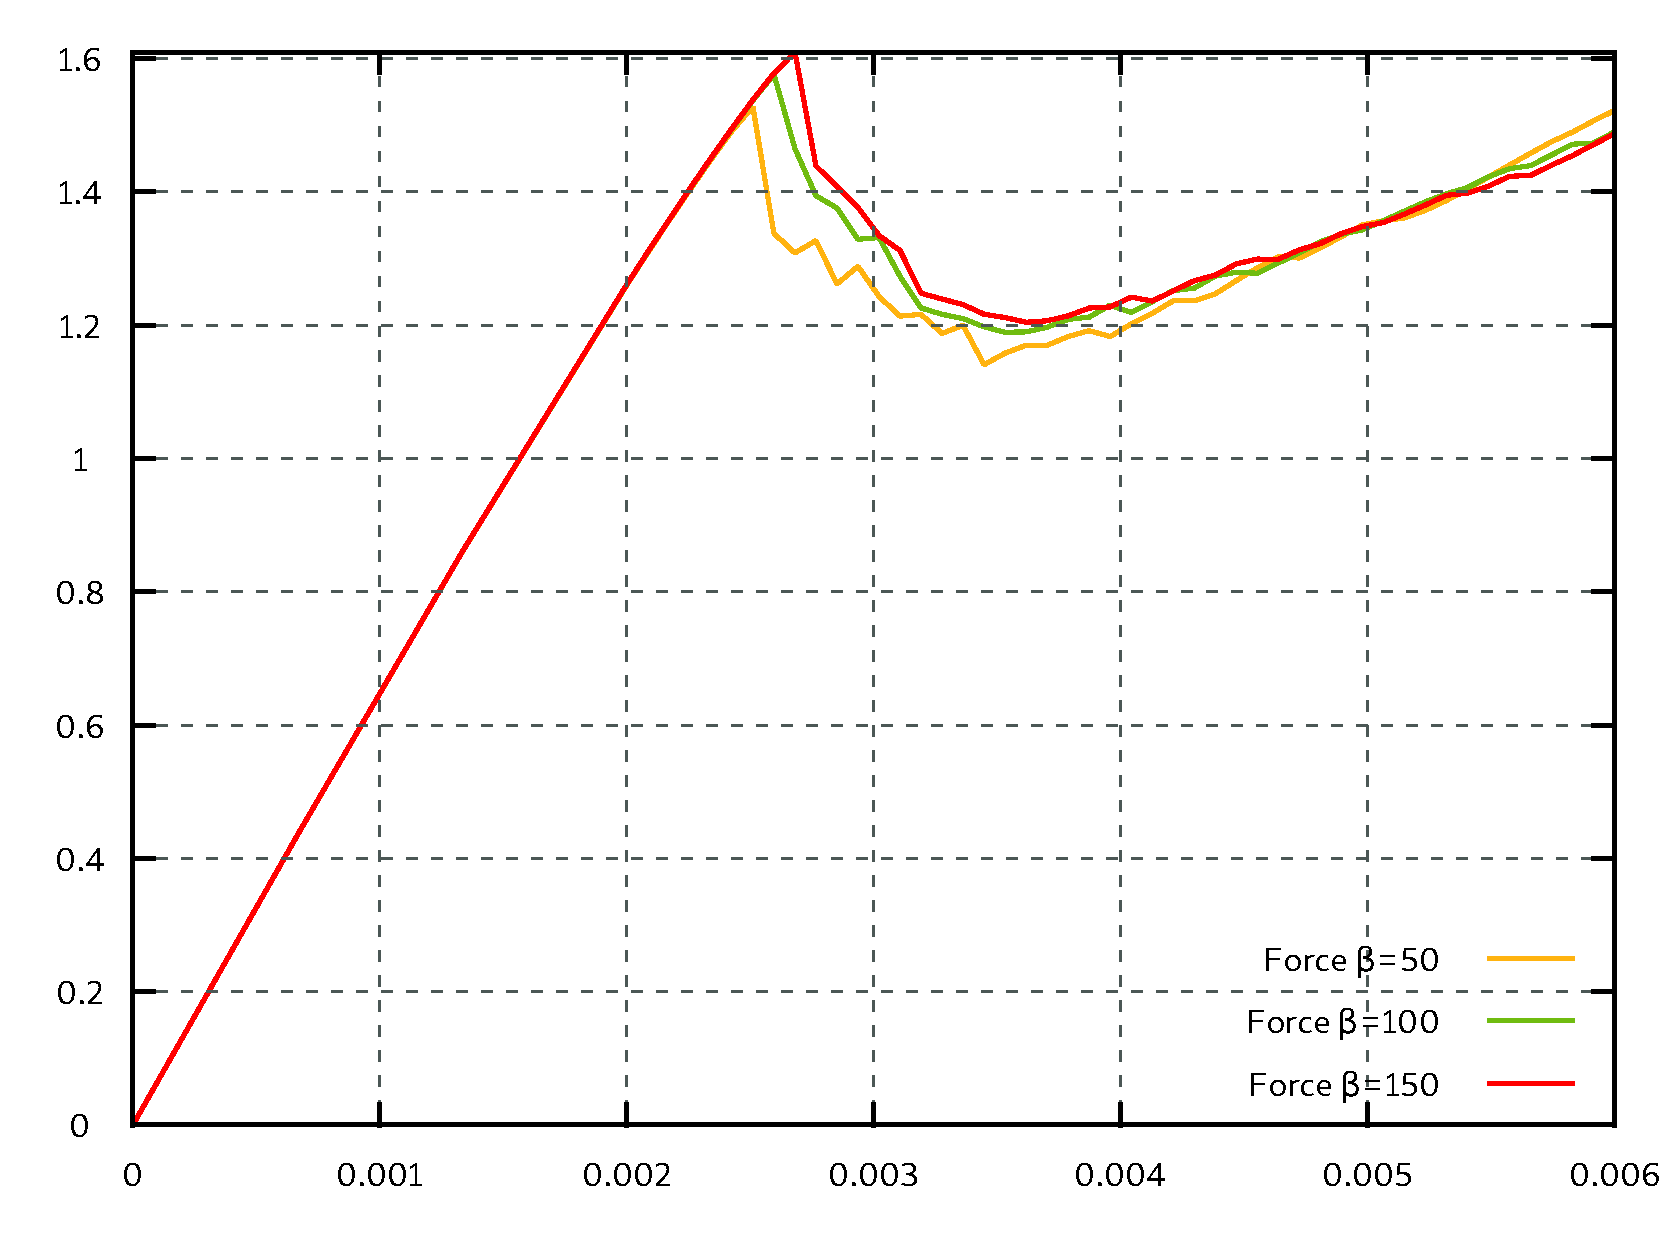
\includegraphics[width=10.cm]{../chapter_02_ef_micromorphic/figures/shear-force.pdf}
  \caption{Evolution of the force as a function of the imposed displacement for
  \(\beta=50\), \(\beta=100\), \(\beta=150\) for the shear test using the
  third staggered scheme}
  \label{fig:micromorphic_damage:beta}
\end{figure}

% ![Evolution of the fracture energy as a function of the imposed
% displacement for \(\beta=50\), \(\beta=100\), \(\beta=150\) for the
% shear test using the third staggered
% scheme.](img/DissipatedEnergies.pdf){width=75%
% #fig:micromorphic_damage:beta2}

\begin{figure}[H]
  \centering
  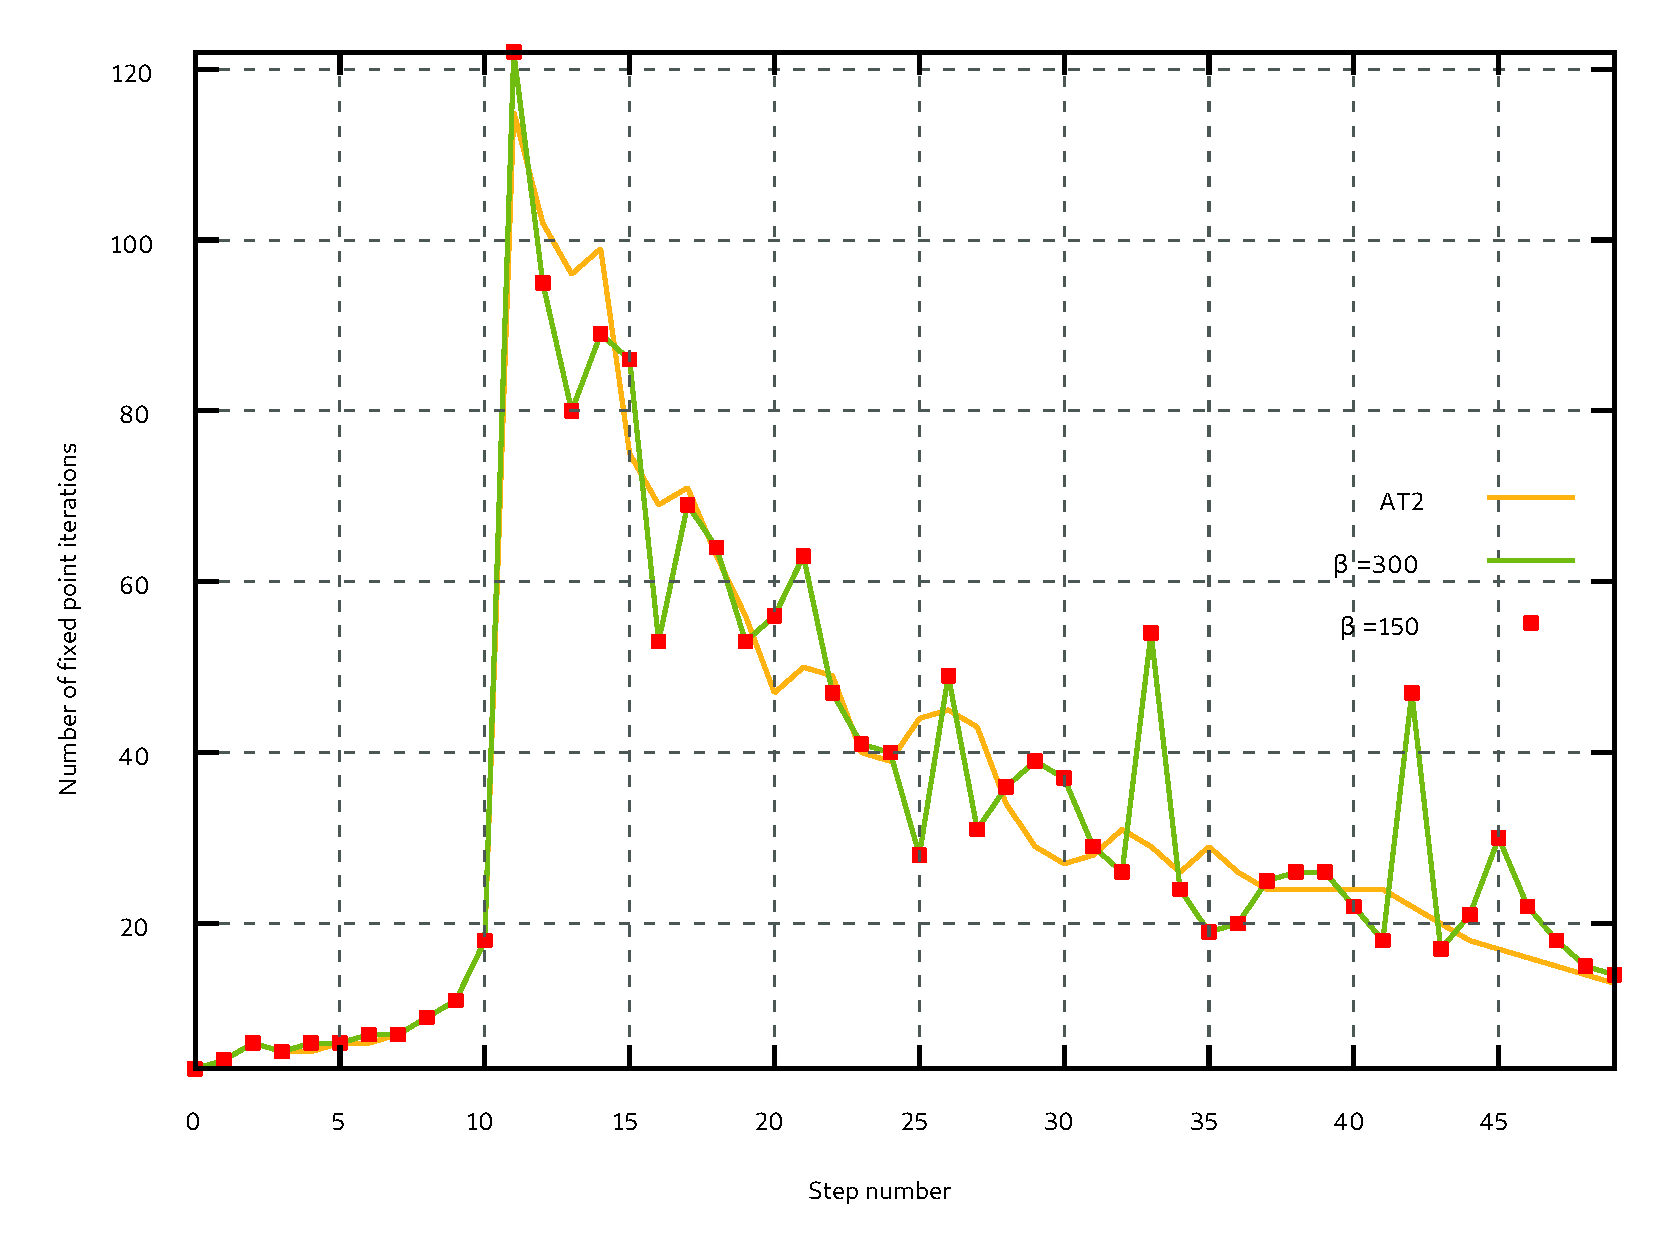
\includegraphics[width=10.cm]{../chapter_02_ef_micromorphic/figures/shear-iterations.pdf}
  \caption{Number of iterations of the fixed point algorithm for the shear test
  as a function of the step number for the standard AT2 model and the
  third scheme for \(\beta=150\) and
  \(\beta=300\)}
  \label{fig:micromorphic_damage:shear:iterations}
\end{figure}

% ![Number of iterations of the fixed point algorithm for the shear test
% as a function of the step number for the standard AT2 model and the
% third scheme for \(\beta=150\) and
% \(\beta=300\).](img/shear-iterations.pdf){width=75%
% #fig:micromorphic_damage:shear:iterations}

\begin{itemize}
  \item The two first schemes converges very slowly (several thousand of fixed
  point iterations) even in the quasi-elastic range. A threshold as
  small as \(10^{-5}\) is required to ensure converged results. Those
  schemes are considered unsuable in pratice.
  \item The third scheme converges much faster. A threshold value of
  \(10^{-3}\) is sufficient to have converged results. The same
  threshold value is used for the standard AT2 model.
  \item As illustrated by Figure \ref{fig:micromorphic_damage:force}, the
  force-displacement curve of the third scheme is very similar to the
  standard AT2 model.
  \item As illustrated by Figure \ref{fig:micromorphic_damage:beta}, the
  penalisation factor plays a major role on the overall
  force-displacement curve. Our experiments shows that a value of
  \(150\) leads to results undistinguishable with the one of the AT2
  model for every tests. However, an higher value of \(300\) is
  required to reproduce closely the evolution of the fracture energy.
  \item The number of iteration of the fixed point algorithm is roughly
  similar between the standard AT2 model and the third scheme, altough a
  bit higher in general, as depicted on Figure
  \ref{fig:micromorphic_damage:shear:iterations}.
\end{itemize}

\subsection{Numerical Experiments}
\label{sec:micromorphicdamage:numerical_experiments}

In this section, the \texttt{MFEM/MGIS} solver is used.

\subsubsection{Shear driven fracture}

Alessi et al. proposed a model to describe deviatoric driven fracture
using the following choice of the elastic free energy
\cite{alessi_phase-field_2020}:
\[
\freeenergyel\paren{\tepsilon, d}=
% \Frac{K}{2}\,\paren{\trace{\tepsilon}}^{2}+
% \mu\,g\paren{d}\,\tenseur{s}^{\varepsilon}\,\colon\,\tenseur{s}^{\varepsilon}
\]
where \(K\) is the bulk modulus, \(\tenseur{s}^{\varepsilon}\) is the
deviatoric part of the elastic strain. The degradation function
\(g\paren{d}\) and the other terms of the Lagrangian are the same as in
the AT2 model.

As stated by Alessi et al., this model lead to quasi-incompressible
behaviour in highly damaged zones and proposed a simple tensile test on
a bar which demonstrated that standard Lagrange elements are not able to
properly describe the damage localisation band and the dissipated energy
by the crack propagation. Alessi et al. then showed that various
classical approaches (selective reduced integration and mixed
displacement/pressure formulation) can overcome this issue.

This test is adapted in this section to demonstrate that the
micromorphic approaches can be used with higher order finite elements.
The same order of approximation will be used to solve the mechanical and
the micromorphic problems.

\subsubsection{Geometry, loadings and meshes}

The specimen is a \(2D\) plate of width \(w\) and height \(h\) treated
under the plane strain hypothesis. The axial displacement of the lower
boundary is set to zero, while the axial displacement of the upper
boundary is imposed. The point at the lower left corner is fixed in the
lateral direction to avoid rigid body motion.

% : Geometry and material parameters for the shear driven fracture test.
% {#tbl:micromorphicdamage:shear_driven_fracture_test_parameters}

% +----------------------------------+-----------------------------+
% | Plate width \(w\)                | \(10^{-3}\, m\)             |
% +----------------------------------+-----------------------------+
% | Plate height \(h\)               | \(2\,\cdot\,10^{-3}\, m\)   |
% +----------------------------------+-----------------------------+
% | Young's modulus \(E\)            | \(210\,\cdot\,10^{9}\, Pa\) |
% +----------------------------------+-----------------------------+
% | Poisson's ratio \(\nu\)          | \(0.3\)                     |
% +----------------------------------+-----------------------------+
% | Fracture energy \(G_{c}\)        | \(2.7\,J.m^{-2}\)           |
% +----------------------------------+-----------------------------+
% | Characteristic length  \(l_{0}\) | \(2.5\,\cdot\,10^{-5}\,m\)  |
% +----------------------------------+-----------------------------+
% | Penalisation factor \(\beta\)    | \(300\)                     |
% +----------------------------------+-----------------------------+

\begin{table}[H]
    \centering
    \begin{tabular}{||c c||} 
        \hline
        Resolution Method & Memory footprint
        \\
        [0.5ex] 
        \hline\hline
        Plate width \(w\)                & \(10^{-3}\, m\)             
        \\ \hline
        Plate height \(h\)               & \(2\,\cdot\,10^{-3}\, m\)   
        \\ \hline
        Young's modulus \(E\)            & \(210\,\cdot\,10^{9}\, Pa\) 
        \\ \hline
        Poisson's ratio \(\nu\)          & \(0.3\)                     
        \\ \hline
        Fracture energy \(G_{c}\)        & \(2.7\,J.m^{-2}\)           
        \\ \hline
        Characteristic length  \(l_{0}\) & \(2.5\,\cdot\,10^{-5}\,m\)  
        \\ \hline
        Penalisation factor \(\beta\)    & \(300\)                     
        \\ \hline
    \end{tabular}
    \caption{Geometry and material parameters for the shear driven fracture test}
    \label{tbl:micromorphicdamage:shear_driven_fracture_test_parameters}
\end{table}


The geometry and the material parameters used for this test are
summarized in Table
\ref{tbl:micromorphicdamage:shear_driven_fracture_test_parameters}. In order
to localize the damage, the fracture energy is assumed uniform in the
plate except in a small square of size \(5\,\cdot\,10^{-2}\,\cdot\,w\)
located at the center of the plate where the fracture energy value is
\(G_{c}\,\cdot\,\paren{1-10^{-2}}\).

: Number of elements for the shear driven fracture test. A very fine
mesh is used for low order finite elements (\(1\) and \(2\)) with
several dozen elements inside the damage band (See Figure
\ref{fig:micromorphicdamage:shear_driven_fracture_test_order1}). A coarser
mesh is used for higher order elements (\(4\) and \(6\)) with \(4\) to
\(6\) elements inside the damage band.

% {#tbl:micromorphicdamage:shear_driven_fracture_test_elements}

% +---------+-----------------------+
% | Order 1 | \(102\,272\) elements |
% +---------+-----------------------+
% | Order 2 | \(409\,088\) elements |
% +---------+-----------------------+
% | Order 4 | \(25\,568\) elements  |
% +---------+-----------------------+
% | Order 6 | \(25\,568\) elements  |
% +---------+-----------------------+

\begin{table}[H]
    \centering
    \begin{tabular}{||c c||} 
        \hline
        Resolution Method & Memory footprint
        \\
        [0.5ex] 
        \hline\hline
        Order 1 & \(102\,272\) elements
        \\ \hline
        Order 2 & \(409\,088\) elements
        \\ \hline
        Order 4 & \(25\,568\) elements 
        \\ \hline
        Order 6 & \(25\,568\) elements 
        \\ \hline
    \end{tabular}
    \caption{Geometry and material parameters for the shear driven fracture test}
    \label{tbl:micromorphicdamage:shear_driven_fracture_test_elements}
\end{table}

The plate is discretized with triangle elements. The number of elements
used as a function of the finite element order is given in Table
\ref{tbl:micromorphicdamage:shear_driven_fracture_test_elements}. In
practice, this number of elements have little influence on the results
and the conclusions drawn in the next paragraph.

\subsection{Results}

\begin{figure}[H]
  \centering
  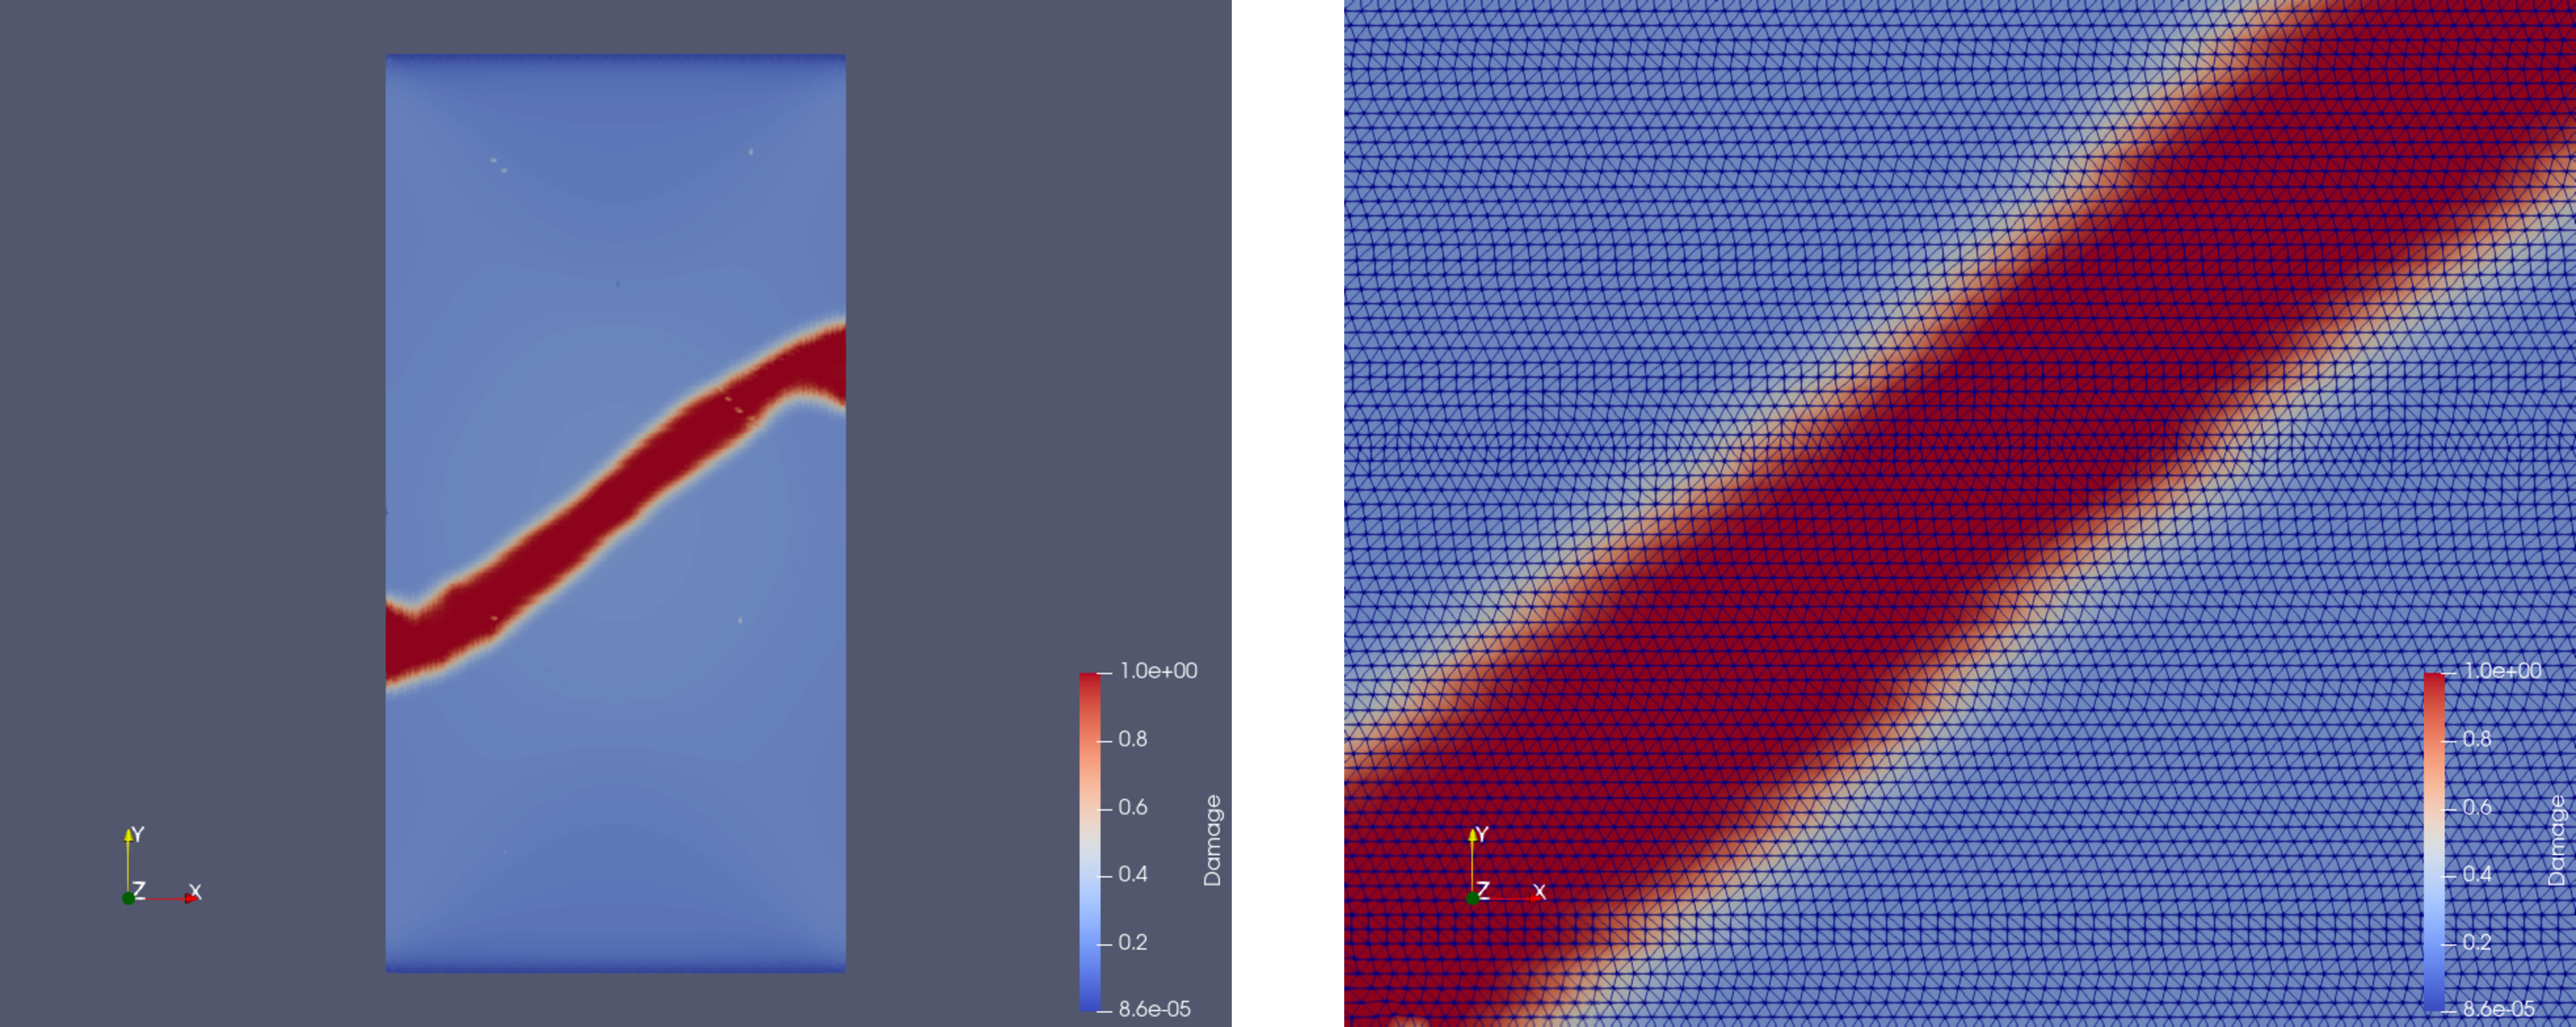
\includegraphics[width=10.cm]{../chapter_02_ef_micromorphic/figures/shear-driven-fracture-damage-results-order-1.pdf}
  \caption{Spurious damage map obtained with linear elements (left). Zoom on the shear fracture (right)}
  \label{fig:micromorphicdamage:shear_driven_fracture_test_order1}
\end{figure}

% ![Spurious damage map obtained with linear elements (left). Zoom on the shear fracture (right)](img/shear-driven-fracture-damage-results-order-1.pdf){#fig:micromorphicdamage:shear_driven_fracture_test_order1 width=75%}

Figure \ref{fig:micromorphicdamage:shear_driven_fracture_test_order1}
describes the damage map pattern after the propagation of the crack. As
described by Alessi et al., volumetric locking leads to a spurious
damage localisation band with excessive thickness, i.e. a thickness
largely greater than the characteristic length \(l_{0}\). A very fine
mesh is used to demonstrate that the issue is not solved by mesh
refinement.

% ![Damage map for higher order elements. Quadradic elements (left), fourth order elements (center), sixth order elements (right). The quadratic mesh is too fine to be shown without hiding the results.](img/shear-driven-fracture-damage-results-higher-orders.pdf){#fig:micromorphicdamage:shear_driven_fracture_test_higher_order width=100%}

\begin{figure}[H]
  \centering
  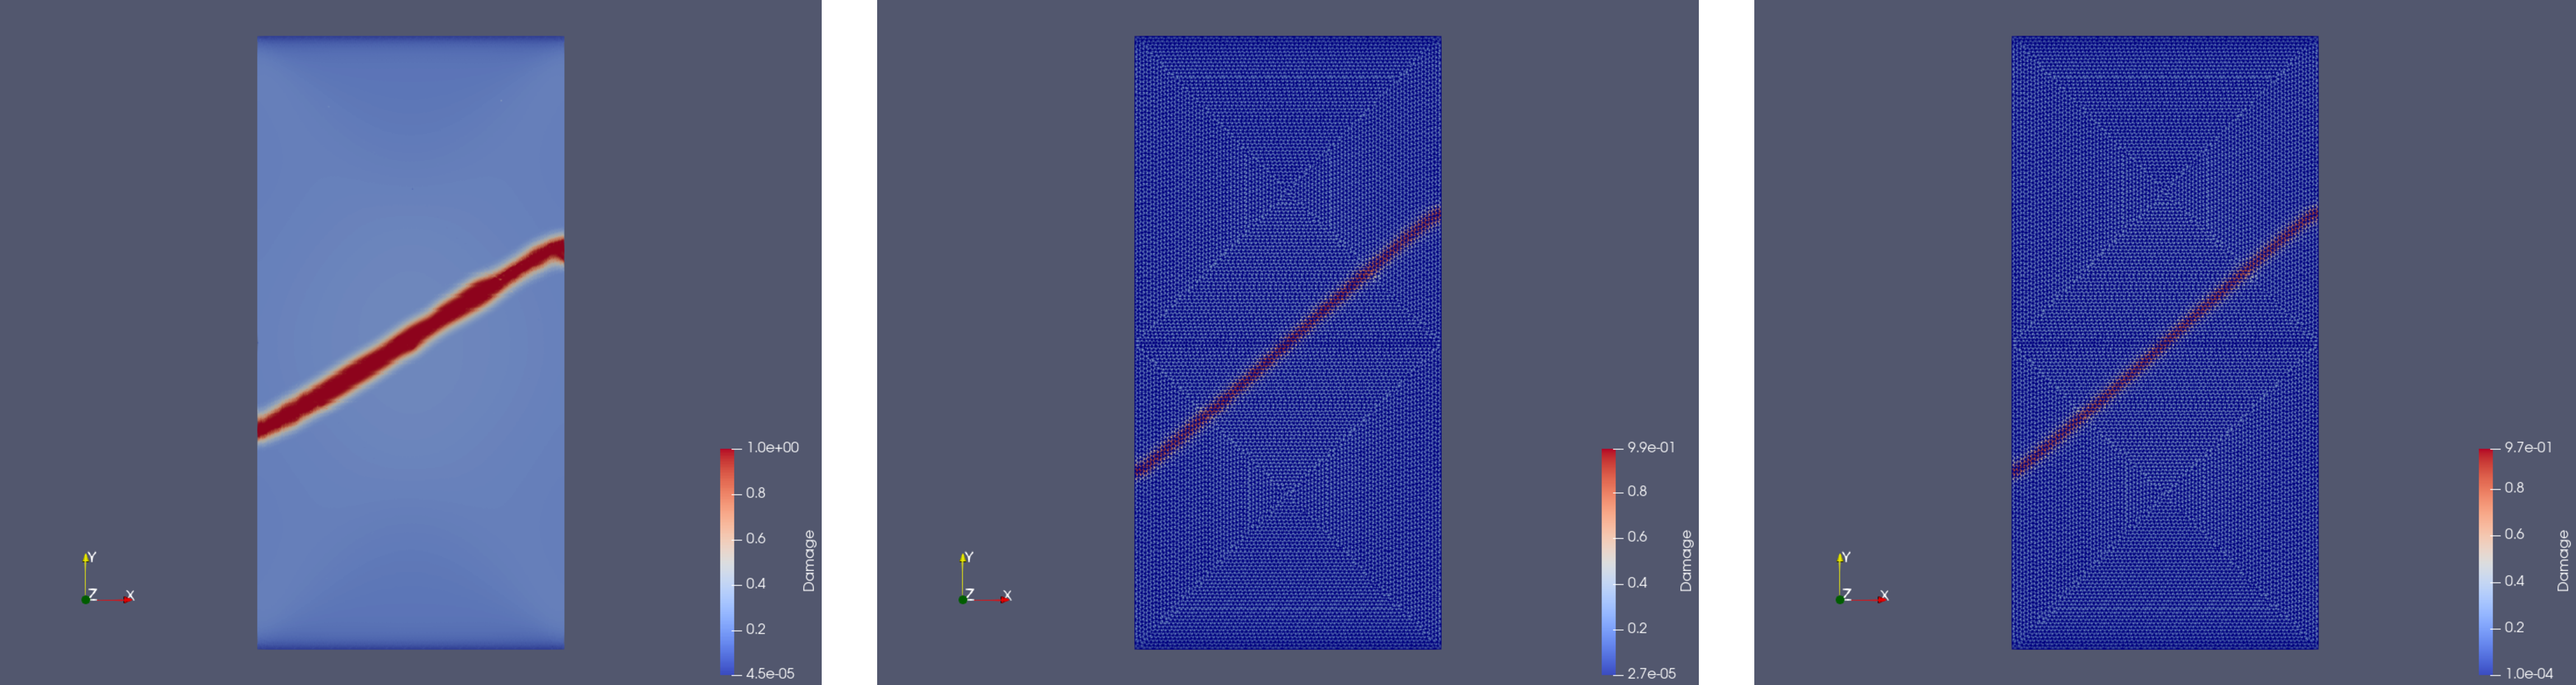
\includegraphics[width=10.cm]{../chapter_02_ef_micromorphic/figures/shear-driven-fracture-damage-results-higher-orders.pdf}
  \caption{Damage map for higher order elements. Quadradic elements (left), fourth order elements (center), sixth order elements (right). The quadratic mesh is too fine to be shown without hiding the results}
  \label{fig:micromorphicdamage:shear_driven_fracture_test_higher_order}
\end{figure}

Figure \ref{fig:micromorphicdamage:shear_driven_fracture_test_higher_order}
show the results obtained with higher order elements. While the
simulation with quadratic elements still exhibit a spurious damage
localisation band, similar to the one observed with linear elements in
Figure \ref{fig:micromorphicdamage:shear_driven_fracture_test_order1}, higher
order elements lead to satisfying results, i.e. higher order elements
alleviate issues related to volumetric locking.

% ![Traction curve](img/shear-driven-fracture-damage-results-force.pdf){#fig:micromorphicdamage:traction_curve width=75%}

\begin{figure}[H]
  \centering
  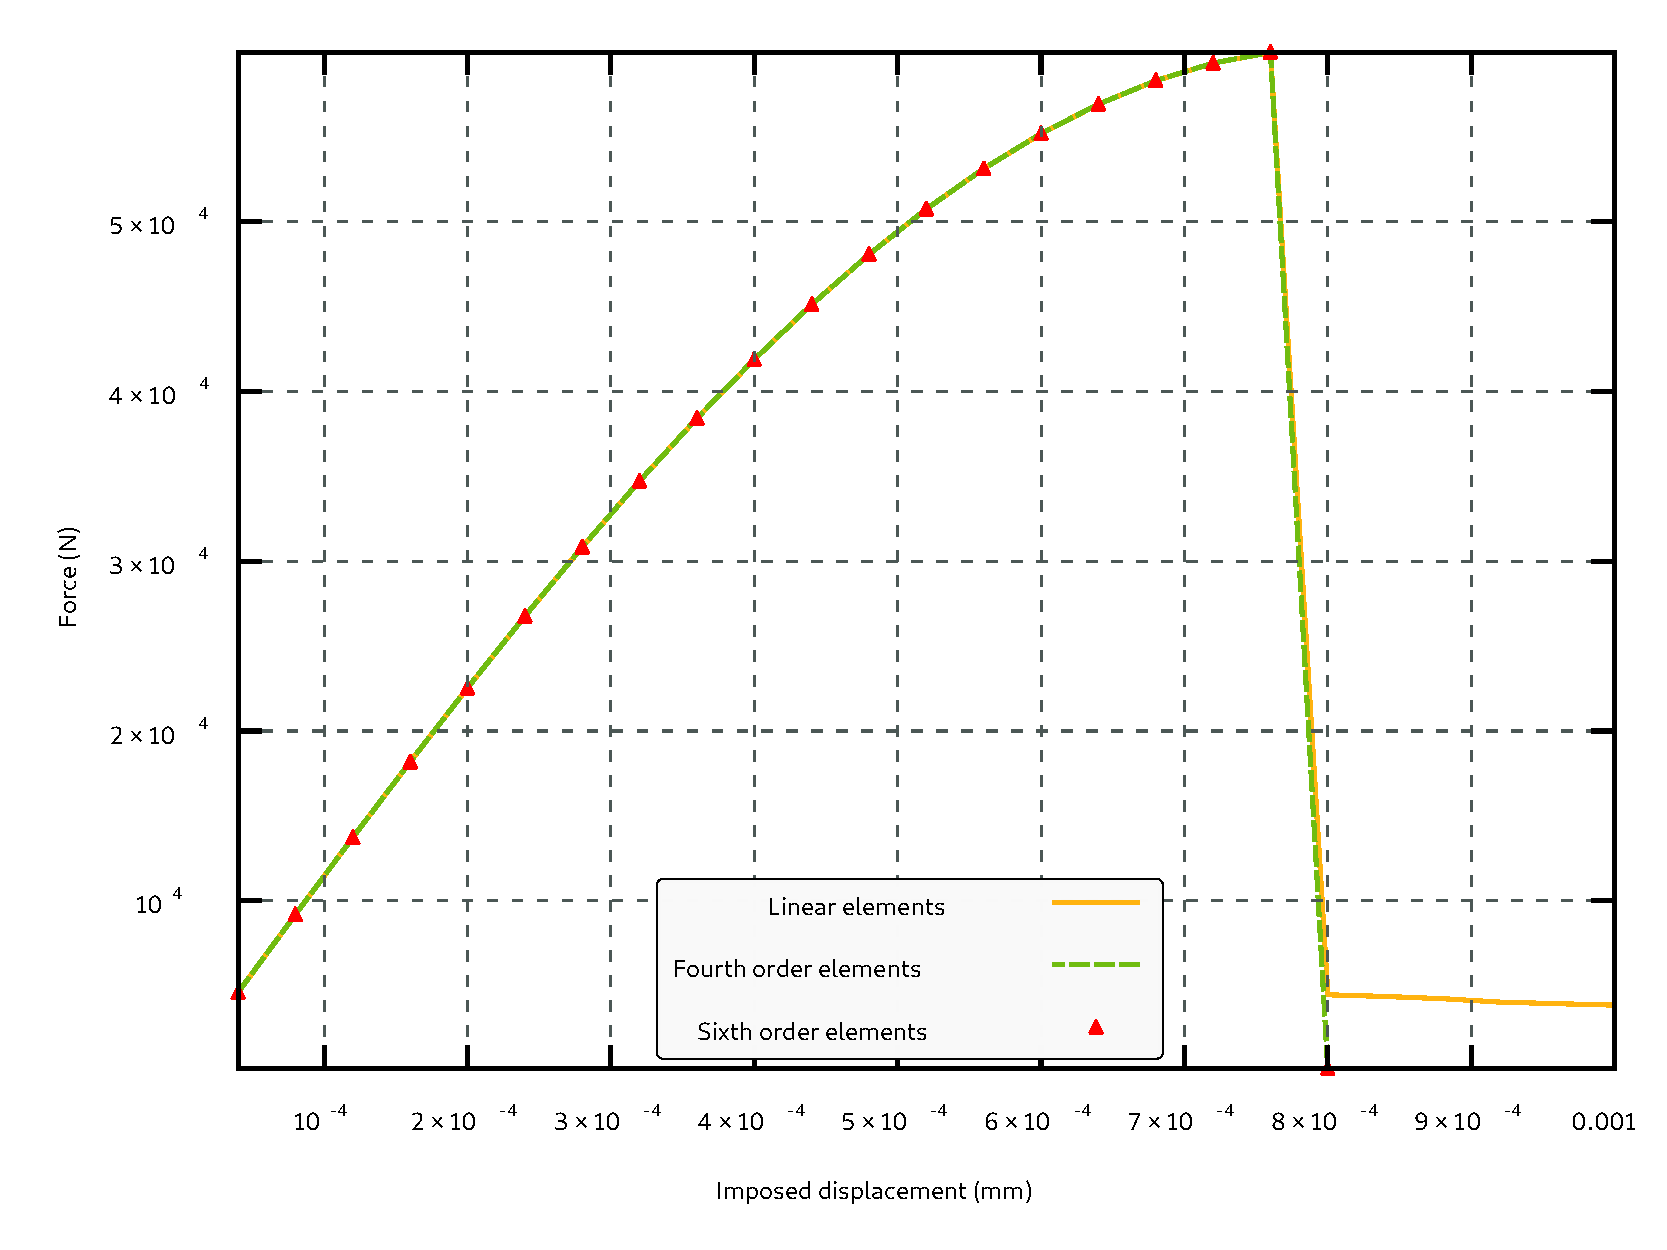
\includegraphics[width=10.cm]{../chapter_02_ef_micromorphic/figures/shear-driven-fracture-damage-results-force.pdf}
  \caption{Traction curve}
  \label{fig:micromorphicdamage:traction_curve}
\end{figure}

Figure \ref{fig:micromorphicdamage:traction_curve} presents the
force/displacement curves as a function of the finite element order.
Quadratic results, which are intermediate between linear and quadratic
results are not reproduced for the sake of clarity. The following
observations can be made:

\begin{itemize}
  \item All order of approximations give similar results up to the crack
  progation.
  \item The traction curve given by linear elements exhibits a residual
  stifness and a spurious dissipation after the crack propagation.
  \item Fourth order and sixth order give undistinguishable results. In both
  cases, the force drops to zero after the crack propagation.
\end{itemize}

\subsection{Industrial test case: nuclear fuel pellet fragmentation}

In this section, the fragmentation of a nuclear fuel pellet during the
reactor start-up. 

\paragraph{Geometry, material and loadings}

% : Geometry, material parameters and loading parameters for the fuel pellet fragementation test.
% {#tbl:micromorphicdamage:fuel_pellet_fragmentation_test_parameters}

% +--------------------------------------------------------------+-----------------------------+
% | Pellet radius \(r_{p}\)                                      | \(4.085\,\cdot\,10^{-3}\)   |
% +--------------------------------------------------------------+-----------------------------+
% | Pellet height \(h_{p}\)                                      | \(6.7\,\cdot\,10^{-3}\)     |
% +--------------------------------------------------------------+-----------------------------+
% | Dishing radius \(r_{d}\)                                     | \(3.05\,\cdot\,10^{-3}\)    |
% +--------------------------------------------------------------+-----------------------------+
% | Dishing height \(h_{d}\)                                     | \(3.2\,\cdot\,10^{-4}\)     |
% +--------------------------------------------------------------+-----------------------------+
% | Young's modulus \(E\)                                        | \(150\,\cdot\,10^{9}\, Pa\) |
% +--------------------------------------------------------------+-----------------------------+
% | Poisson's ratio \(\nu\)                                      | \(0.3\)                     |
% +--------------------------------------------------------------+-----------------------------+
% | Linear mean thermal expansion coefficient \(\alpha\)         | \(1\,\cdot\,10^{-5}\)       |
% +--------------------------------------------------------------+-----------------------------+
% | Thermal expansion reference temperature \(T_{\mathrm{ref}}\) | \(1\,\cdot\,10^{-5}\)       |
% +--------------------------------------------------------------+-----------------------------+
% | Fracture energy \(G_{c}\)                                    | \(xxx\,J.m^{-2}\)           |
% +--------------------------------------------------------------+-----------------------------+
% | Characteristic length  \(l_{0}\)                             | \(xxx\,\cdot\,10^{-xx}\,m\) |
% +--------------------------------------------------------------+-----------------------------+
% | Penalisation factor \(\beta\)                                | \(300\)                     |
% +--------------------------------------------------------------+-----------------------------+
% | Core temperature\(T_{c}\)                                    | \(1500\,K\)                 |
% +--------------------------------------------------------------+-----------------------------+
% | Outer surface temperature \(T_{o}\)                          | \(600\,K\)                  |
% +--------------------------------------------------------------+-----------------------------+

\begin{table}[H]
    \centering
    \begin{tabular}{||c c||} 
        \hline
        Resolution Method & Memory footprint
        \\
        [0.5ex] 
        \hline\hline
        Pellet radius \(r_{p}\)                                      & \(4.085\,\cdot\,10^{-3}\)   
        \\ \hline
        Pellet height \(h_{p}\)                                      & \(6.7\,\cdot\,10^{-3}\)     
        \\ \hline
        Dishing radius \(r_{d}\)                                     & \(3.05\,\cdot\,10^{-3}\)    
        \\ \hline
        Dishing height \(h_{d}\)                                     & \(3.2\,\cdot\,10^{-4}\)     
        \\ \hline
        Young's modulus \(E\)                                        & \(150\,\cdot\,10^{9}\, Pa\) 
        \\ \hline
        Poisson's ratio \(\nu\)                                      & \(0.3\)                     
        \\ \hline
        Linear mean thermal expansion coefficient \(\alpha\)         & \(1\,\cdot\,10^{-5}\)       
        \\ \hline
        Thermal expansion reference temperature \(T_{\mathrm{ref}}\) & \(1\,\cdot\,10^{-5}\)       
        \\ \hline
        Fracture energy \(G_{c}\)                                    & \(xxx\,J.m^{-2}\)           
        \\ \hline
        Characteristic length  \(l_{0}\)                             & \(xxx\,\cdot\,10^{-xx}\,m\) 
        \\ \hline
        Penalisation factor \(\beta\)                                & \(300\)                     
        \\ \hline
        Core temperature\(T_{c}\)                                    & \(1500\,K\)                 
        \\ \hline
        Outer surface temperature \(T_{o}\)                          & \(600\,K\)            
        \\ \hline
    \end{tabular}
    \caption{Geometry, material parameters and loading parameters for the fuel pellet fragementation test}
    \label{tbl:micromorphicdamage:fuel_pellet_fragmentation_test_parameters}
\end{table}

\subsection{Thermal expansion}

The strain \(\tepsilonth\) associated with the thermal expansion is
computed as follows:
\[
\tepsilonth\paren{T}=\alpha\,\paren{T-T_{\mathrm{ref}}}\,\tenseur{I}
\]
where:

- \(T\) is the temperature.
- \(T_{\mathrm{ref}}\) is a reference temperature.
- \(\alpha\) is the mean linear thermal expansion coefficient.

\subsection{Modification of the free energy}

To take thermal expansion into account, the free energy
\(\freeenergyel\paren{\tepsilon, d}\) is modified as follows:

\begin{equation}
  \label{eq:micromorphicdamage:freeenergygel}
  \freeenergyel\paren{\tepsilon, T, d} = 
  g\paren{d}\,\freeenergyel_{0}\paren{\tepsilon-\tepsilonth} =
  \Frac{g\paren{d}}{2}\,\paren{\tepsilon-\tepsilonth}\,\colon\,\tenseurq{D}\,\colon\,\paren{\tepsilon-\tepsilonth}
\end{equation}

% \[
% \freeenergyel\paren{\tepsilon, T, d} = 
% g\paren{d}\,\freeenergyel_{0}\paren{\tepsilon-\tepsilonth} =
% \Frac{g\paren{d}}{2}\,\paren{\tepsilon-\tepsilonth}\,\colon\,\tenseurq{D}\,\colon\,\paren{\tepsilon-\tepsilonth}
% \]{#eq:micromorphicdamage:freeenergygel}

\subsection{Temperature profile}

Under the approximation of a constant thermal conductivity, the
temperature profile in a PWR fuel pellet is axisymmetric and parabolic:
\[
T\paren{r, t}=\Delta\,T\paren{t}\,\paren{1-r^{2}}+T_{\mathrm{o}}
\]
where:

\begin{itemize}
  \item \(t\) is a loading parameter in the range \([0:1]\).
  \item \(T_{\mathrm{o}}\) is the temperature at the outer boundary of the
    fuel pellet.
  \item The temperature increase \(\Delta\,T\paren{t}\) is chosen as a linear
    function of the loading parameter as follows:
    \[
    \Delta\,T\paren{t} = \paren{T_{\mathrm{c}}-T_{\mathrm{o}}}\, t
    \]
\end{itemize}

\subsection{Results}

\(33\,230\,848\) triangles, \(132'923'392\) nodes, \(4.10^8\) degrees of freedom for the mechanical problem.

% ![Crack pattern](img/FuelPelletCracking-results.pdf){width=75%}

\begin{figure}[H]
  \centering
  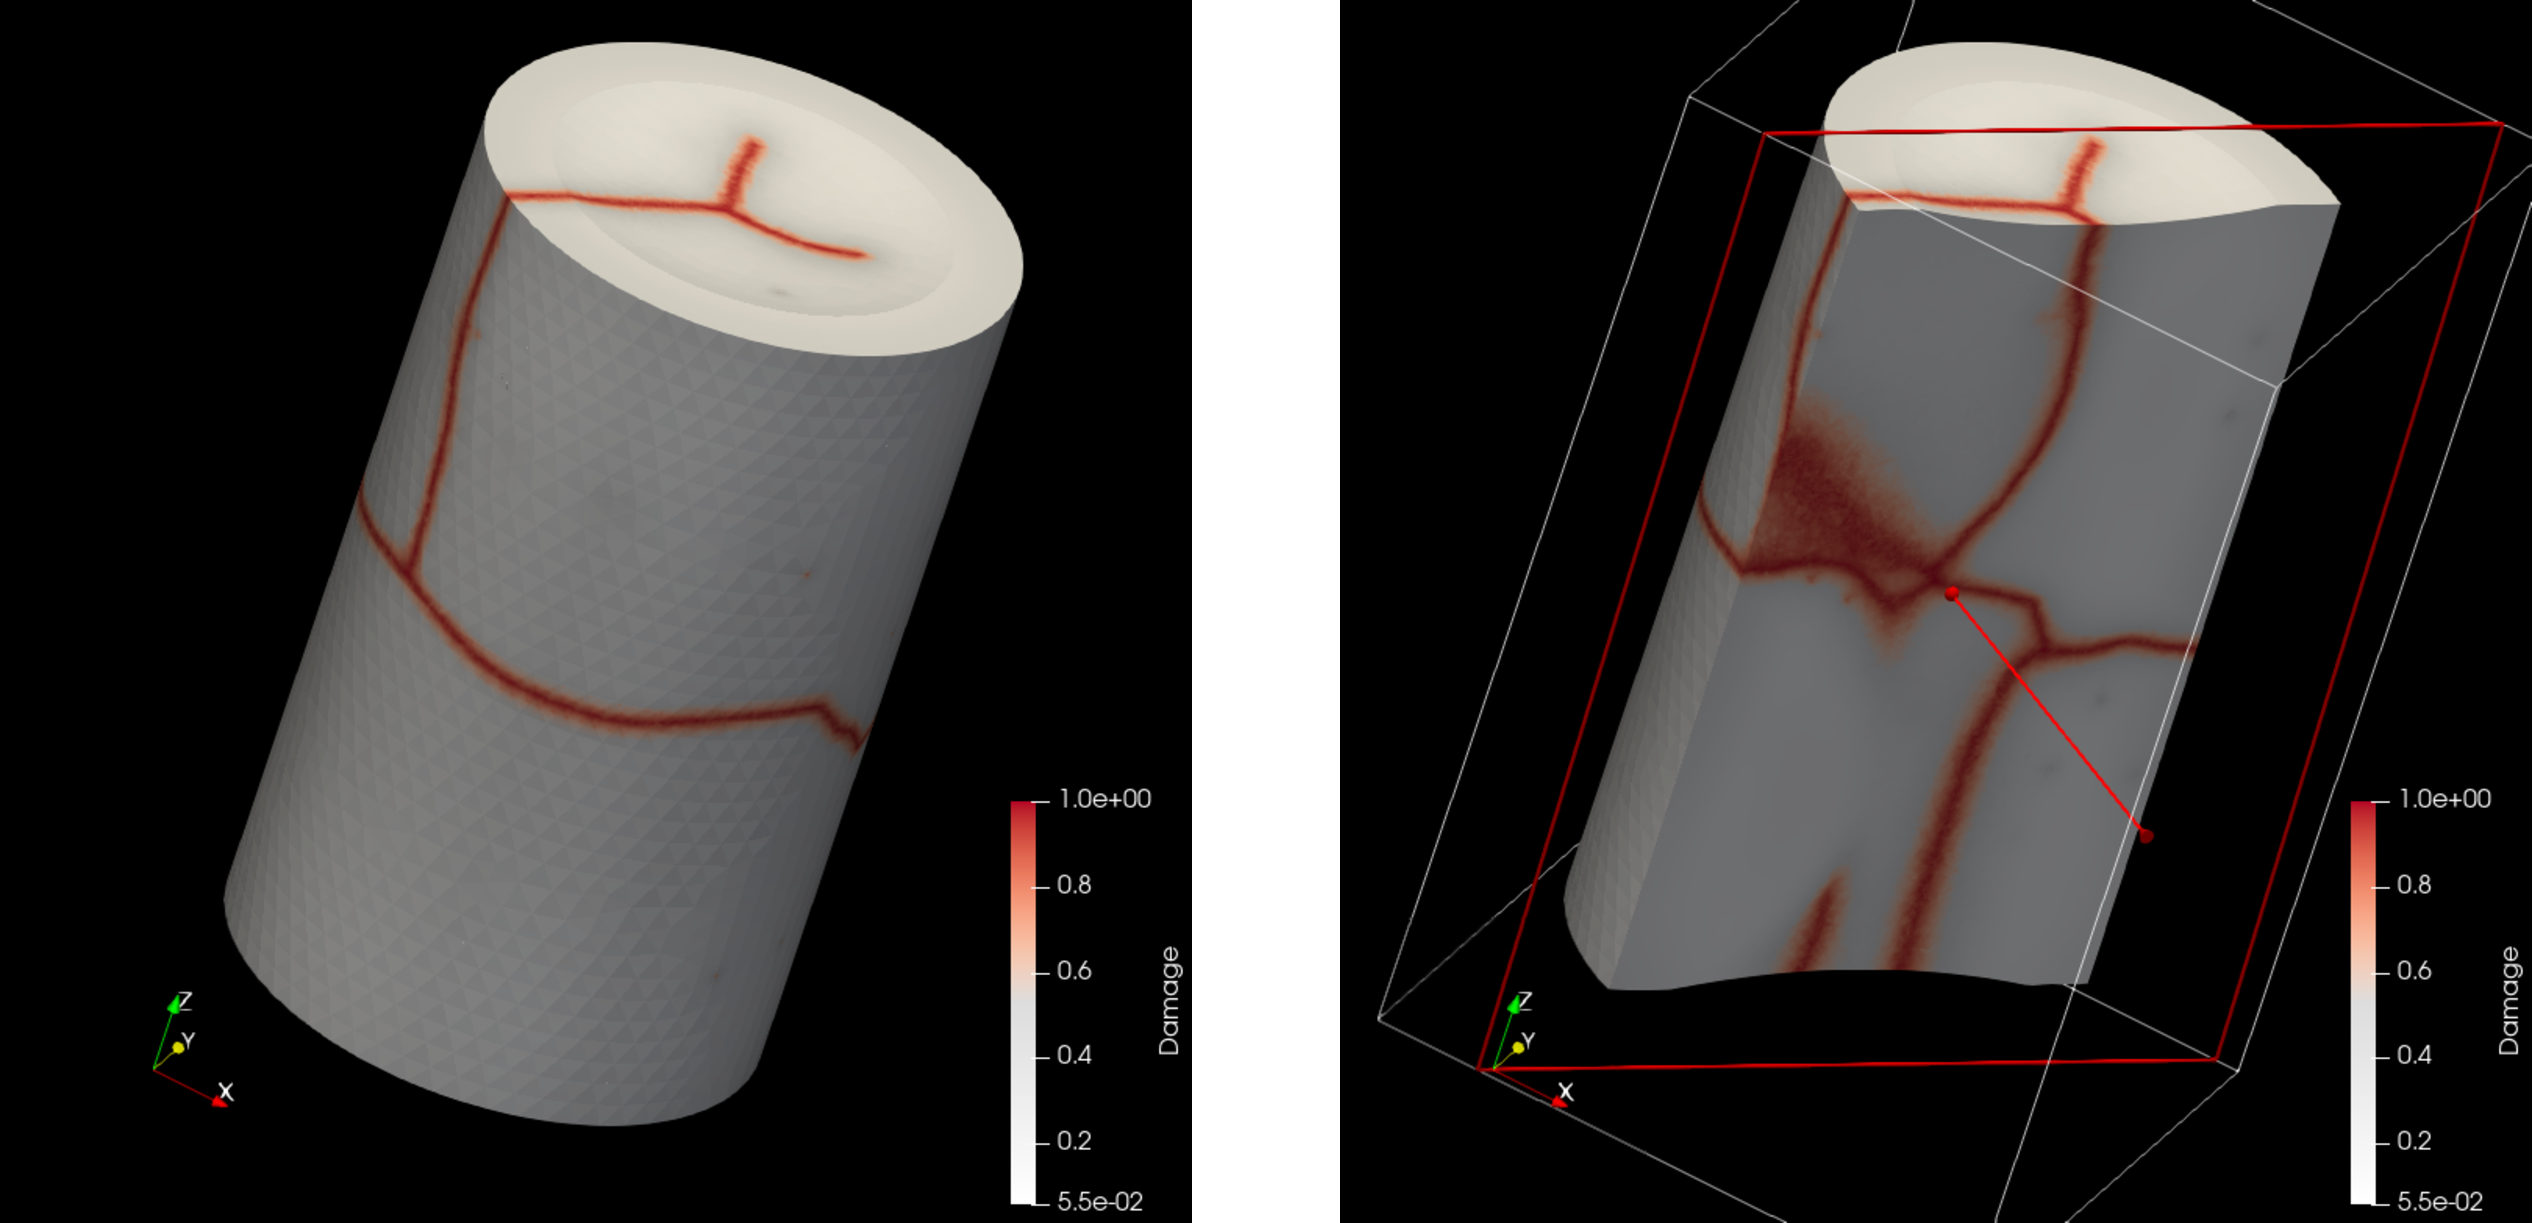
\includegraphics[width=10.cm]{../chapter_02_ef_micromorphic/figures/FuelPelletCracking-results.pdf}
  \caption{Crack pattern}
\end{figure}
